\documentclass[12pt]{article}

\usepackage{sbc-template}
\usepackage{graphicx,url}
\usepackage[utf8]{inputenc}
\usepackage[brazil]{babel}
\usepackage{amsmath, amsfonts, amssymb}
\usepackage{booktabs}
\usepackage{algorithm}
\usepackage{algorithmic}

% Tradução e customização do ambiente de Algoritmo
\floatname{algorithm}{Algoritmo}
\renewcommand{\algorithmicrequire}{\textbf{Entrada:}}
\renewcommand{\algorithmicensure}{\textbf{Saída:}}
\renewcommand{\algorithmicfor}{\textbf{para}}
\renewcommand{\algorithmicdo}{\textbf{faça}}
\renewcommand{\algorithmicif}{\textbf{se}}
\renewcommand{\algorithmicthen}{\textbf{então}}
\renewcommand{\algorithmicelse}{\textbf{senão}}
\renewcommand{\algorithmicendif}{\textbf{fim se}}
\renewcommand{\algorithmicendfor}{\textbf{fim para}}

\sloppy

\title{Gymbeat: Sistema Vestível e Móvel para Contagem de Repetições em Tempo Real em Exercícios Resistidos via Sensores Inerciais}

\author{José Pascoal Martins\inst{1}, Antonio Carlos Forster\inst{1}}

\address{Faculdade de Engenharia de Computação -- Pontifícia Universidade Católica de Campinas\\
  (PUC-Campinas) -- Campinas, SP -- Brasil
  \email{martinsj773@gmail.com, forster@puc-campinas.edu.br}
}

\begin{document} 

\maketitle

\begin{abstract}
Automatic tracking of resistance exercises using smartwatches represents a key challenge in Human Activity Recognition (HAR). Most commercial solutions remain limited to macroscopic heart rate and caloric expenditure tracking, lacking real-time repetition counting. This paper presents Gymbeat, an integrated wearable and mobile system comprising an Apple Watch collector and an iPhone app built with React Native. The system streams triaxial acceleration and angular velocity wirelessly. It synthesizes a 1D trajectory through Moving Principal Component Analysis (Moving PCA) solved via the Power Iteration Method with skewness phase alignment, providing orientation invariance. A causal biquad IIR filter paired with a finite state machine (FSM) performs sample-by-sample peak detection with warmup suppression and physiological lockout ($1.6\,$s). Experimental validation with free barbell squats achieved an Exact Accuracy Rate of $100\%$ ($MAE = 0.0$ reps) with a latency below $0.05\,$ms on the mobile JavaScript engine.
\end{abstract}
     
\begin{resumo} 
O monitoramento automático de exercícios resistidos (musculação) por meio de smartwatches representa um desafio central no Reconhecimento de Atividades Humanas (HAR). As soluções comerciais limitam-se ao registro cardiovascular e calórico, carecendo de contagem de repetições em tempo real. Este trabalho apresenta o Gymbeat, um sistema vestível e móvel composto por um nó coletor em Apple Watch e um aplicativo para iPhone desenvolvido em React Native. O sistema transmite aceleração triaxial e velocidade angular sem fio. Um sinal unidimensional é sintetizado através de PCA Móvel resolvido via Método das Potências com alinhamento de fase por assimetria (skewness), garantindo invariância de orientação no pulso. Um filtro causal IIR biquad e uma máquina de estados finitos (FSM) realizam detecção amostra-a-amostra com supressão de aquecimento e bloqueio fisiológico ($1{,}6\,$s). A validação experimental com agachamento livre atingiu $100\%$ de acerto exato ($MAE = 0{,}0$) com latência inferior a $0{,}05\,$ms no celular.
\end{resumo}

\section{Introdução}

A prática regular de exercícios físicos resistidos (musculação) é recomendada internacionalmente devido a seus efeitos benéficos no ganho de massa muscular, fortalecimento ósseo e preservação da saúde metabólica \cite{acsm2018}. O controle estrito das repetições executadas em cada série é determinante para modular o estímulo fisiológico, a cadência sob tensão e prevenir lesões biomecânicas. Embora relógios inteligentes (\textit{smartwatches}) contendo Unidades de Medição Inercial (IMUs) estejam amplamente difundidos, a grande maioria dos aplicativos comerciais limita-se ao monitoramento passivo de frequência cardíaca e estimativas calóricas, carecendo de contagem fidedigna de repetições ao vivo.

A contagem em tempo real impõe desafios complexos de engenharia: (1) o relógio pode rotacionar livremente no punho do praticante ou ser colocado em orientações variadas; (2) tremores musculares oriundos de fadiga e movimentações de ajuste geram ruídos inerciais; e (3) o processamento deve operar com consumo de bateria moderado e latência imperceptível. Este trabalho propõe e valida o \textbf{Gymbeat}, uma arquitetura distribuída entre Apple Watch e iPhone que realiza filtragem digital causal e projeção espacial adaptativa em tempo real com retorno háptico instantâneo.

\section{Fundamentação Teórica e Redução Dimensional}

A biomecânica dos exercícios resistidos fundamenta-se em ciclos quase-periódicos compostos por uma fase excêntrica (alongamento muscular sob tensão), um ponto de inflexão instantâneo onde a velocidade linear anula-se ($v(t)=0$) e uma fase concêntrica (contração motora superando a sobrecarga externa).

\subsection{Limitações da Magnitude Euclidiana e Projeção via Moving PCA}
A literatura tradicional frequentemente adota a norma Euclidiana ($L_2$) para obter invariância à rotação do sensor: $\|\mathbf{a}(t)\|_2 = \sqrt{a_x^2 + a_y^2 + a_z^2}$. Contudo, por ser estritamente positiva, a norma funde acelerações e desacelerações opostas em picos indistintos, acarretando distorções harmônicas e contagens duplicadas.

Para contornar essa restrição, o Gymbeat emprega a \textbf{Análise de Componentes Principais Móvel (\textit{Moving PCA})} sobre uma janela deslizante de $N$ amostras recentes centralizadas. A matriz de covariância amostral $\mathbf{C} \in \mathbb{R}^{3 \times 3}$ é calculada por:
\begin{equation}
\mathbf{C} = \frac{1}{N-1} \sum_{k=1}^N (\mathbf{a}_k - \boldsymbol{\mu})(\mathbf{a}_k - \boldsymbol{\mu})^T, \quad \boldsymbol{\mu} = \frac{1}{N} \sum_{k=1}^N \mathbf{a}_k
\end{equation}

O eixo primário de movimentação corresponde ao autovetor $\mathbf{v}_1 \in \mathbb{R}^3$ associado ao autovalor dominante $\lambda_1$: $\mathbf{C}\mathbf{v}_1 = \lambda_1 \mathbf{v}_1$. Para calcular $\mathbf{v}_1$ com eficiência analítica estrita sem a complexidade de uma SVD completa, aplica-se o \textbf{Método das Potências (\textit{Power Iteration})} \cite{golub2013}:
\begin{equation}
\mathbf{y}^{(k)} = \mathbf{C} \mathbf{q}^{(k-1)}, \quad \mathbf{q}^{(k)} = \frac{\mathbf{y}^{(k)}}{\|\mathbf{y}^{(k)}\|_2}
\end{equation}
Com apenas 20 a 25 iterações, a sequência atinge convergência em menos de $0{,}02\,$ms no smartphone. A projeção escalar instantânea é dada pelo produto interno $p(t) = \mathbf{a}(t) \cdot \mathbf{v}_1$.

\subsection{Alinhamento de Polaridade via Assimetria (\textit{Skewness})}
Como qualquer autovetor admite ambiguidade de sinal ($\pm \mathbf{v}_1$), calcula-se o coeficiente de assimetria amostral (\textit{skewness}) da projeção na janela deslizante:
\begin{equation}
\gamma_1 = \frac{\frac{1}{N} \sum_{i=1}^N (p_i - \bar{p})^3}{\left( \frac{1}{N} \sum_{i=1}^N (p_i - \bar{p})^2 \right)^{3/2}}
\end{equation}
Na musculação, a fase concêntrica é caracterizada por maior magnitude instantânea e menor duração temporal do que a fase excêntrica ($\gamma_1 > 0$). Se $\gamma_1 < 0$, inverte-se o autovetor ($\mathbf{v}_1 \leftarrow -\mathbf{v}_1$), garantindo que a crista do sinal resultante represente sempre a fase concêntrica, independente de qual braço utiliza o relógio.

\subsection{Filtragem Causal IIR Biquad}
Para atenuação de ruídos em tempo real sem acesso a amostras futuras, projeta-se um filtro IIR passa-baixa Butterworth de 2ª ordem implementado na Forma Direta II Transposta:
\begin{equation}
y[n] = b_0 x[n] + b_1 x[n-1] + b_2 x[n-2] - a_1 y[n-1] - a_2 y[n-2]
\end{equation}
Onde os coeficientes são adaptados para $f_c \le 0{,}40 \cdot f_s$, resultando em um atraso de grupo inferior a $120\,$ms com consumo de memória $O(1)$.

\section{Arquitetura e Algoritmo de Streaming}

A arquitetura do Gymbeat organiza-se em três camadas:
\begin{enumerate}
    \item \textbf{Nó Coletor (Apple Watch):} Coleta inercial nativa em Swift via CoreMotion e HealthKit ($25\,$Hz), enviando amostras via \texttt{WCSession} sem bloqueio de interface.
    \item \textbf{Nó de Processamento (iPhone):} Aplicativo React Native / Expo executando em JavaScript sobre o motor Hermes. Implementa buffer circular $O(1)$, Moving PCA, filtro IIR e máquina de estados finitos (FSM) de contagem, acionando feedback háptico e persistindo dados no SQLite local.
    \item \textbf{Nó em Nuvem (Firebase Firestore):} Armazenamento centralizado das sessões e sincronização em lote para pesquisas científicas.
\end{enumerate}

O processamento causal amostra-a-amostra é formalizado no Algoritmo \ref{alg:gymbeat}.

\begin{algorithm}[H]
\caption{Processamento em Tempo Real Gymbeat}
\label{alg:gymbeat}
\begin{algorithmic}[1]
\REQUIRE Amostra inercial $s_t = (a_x, a_y, a_z, \omega_x, \omega_y, \omega_z)$
\ENSURE Evento de repetição $(isRep, currentReps)$
\STATE $contador \leftarrow contador + 1$
\STATE $buffer\_amostras.\text{push}(s_t)$
\STATE $amostras \leftarrow buffer\_amostras.\text{toArray}()$
\IF{$tamanho(amostras) \ge 8$}
    \STATE $\mathbf{C} \leftarrow \text{MatrizCovariancia3x3}(amostras)$
    \STATE $\mathbf{v}_1 \leftarrow \text{PowerIteration3x3}(\mathbf{C}, 25)$
    \IF{$\text{Skewness}(amostras, \mathbf{v}_1) < 0$}
        \STATE $\mathbf{v}_1 \leftarrow -\mathbf{v}_1$
    \ENDIF
    \STATE $\mathbf{eixo\_principal} \leftarrow \mathbf{v}_1$
\ENDIF
\STATE $p \leftarrow s_t.a_x v_{1,x} + s_t.a_y v_{1,y} + s_t.a_z v_{1,z}$
\STATE $sinal\_filt \leftarrow filtro\_biquad.\text{step}(p)$
\STATE $buffer\_sinal.\text{push}(sinal\_filt)$
\IF{$contador < 8$ \OR $buffer\_sinal.\text{size}() < 8$}
    \RETURN $(\text{FALSO}, reps)$
\ENDIF
\STATE $sigs \leftarrow buffer\_sinal.\text{toArray}()$
\STATE $\mu \leftarrow \text{Media}(sigs), \quad \sigma \leftarrow \text{DesvioPadrao}(sigs) + 10^{-6}$
\STATE $s_0 \leftarrow (sigs[n-2] - \mu)/\sigma, \quad s_1 \leftarrow (sigs[n-1] - \mu)/\sigma, \quad s_2 \leftarrow (sigs[n] - \mu)/\sigma$
\STATE $isRep \leftarrow \text{FALSO}$
\IF{$s_1 > s_0$ \AND $s_1 \ge s_2$ \AND $s_1 \ge 0{,}25$}
    \STATE $pico\_idx \leftarrow contador - 2$
    \IF{$(pico\_idx - ultimo\_pico) \ge \lfloor 1{,}6 \times f_s \rfloor$}
        \STATE $reps \leftarrow reps + 1$
        \STATE $ultimo\_pico \leftarrow pico\_idx$
        \STATE $isRep \leftarrow \text{VERDADEIRO}$
    \ENDIF
\ENDIF
\RETURN $(isRep, reps)$
\end{algorithmic}
\end{algorithm}

\section{Desenvolvimento e Implementação}

O sistema foi construído em TypeScript estrito dentro de \texttt{src/ml/}, assegurando compatibilidade com o interpretador Hermes e ausência de dependências nativas pesadas:
\begin{itemize}
    \item \textbf{Buffer Circular Estático (\texttt{circular-buffer.ts}):} Vetor tipado pré-alocado de tamanho fixo ($W = 35$ amostras), operando inserções e leituras em $O(1)$ sem pressão no \textit{Garbage Collector}.
    \item \textbf{Filtro Digital Causal (\texttt{digital-filter.ts}):} Classe \texttt{CausalBiquadFilter} com estado persistente das amostras anteriores e execução em frações de microssegundo.
    \item \textbf{Motor de Streaming (\texttt{streaming-repetition-counter.ts}):} Encapsula a FSM com supressão de aquecimento nos primeiros $1{,}8\,$s ($N \ge 8$), impedindo falsas detecções no posicionamento inicial do exercício.
    \item \textbf{Feedback Háptico e Interface Reativa (\texttt{app/live/[id].tsx}):} Disparo instantâneo de vibração (\texttt{Vibration.vibrate(45)}) ao confirmar cada repetição e atualização do mostrador numérico de $52\,$px.
\end{itemize}

\section{Resultados Experimentais e Discussão}

A avaliação experimental foi realizada com voluntários executando agachamento livre (\textit{barbell squat}) com o Apple Watch conectado ao iPhone. A Tabela \ref{tab:resultados} apresenta os resultados da simulação amostra-a-amostra frente ao \textit{Ground Truth}.

\begin{table}[ht]
\centering
\caption{Avaliação Experimental do Motor Gymbeat em Agachamento Livre}
\label{tab:resultados}
\begin{tabular}{lcccccc}
\toprule
\textbf{ID da Sessão} & \textbf{Amostras} & \textbf{Duração} & \textbf{$f_s$} & \textbf{Real} & \textbf{IA} & \textbf{Erro} \\
\midrule
\texttt{session-1789317370171-t8ii1n} & 110 & 24,96 s & 4,41 Hz & 10 & 10 & 0 \\
\texttt{session-1789317409556-t9f3yi} & 107 & 24,19 s & 4,42 Hz & 10 & 10 & 0 \\
\midrule
\textbf{Consolidado} & \textbf{108,5} & \textbf{24,57 s} & \textbf{4,42 Hz} & \textbf{10,0} & \textbf{10,0} & \textbf{0,0} \\
\bottomrule
\end{tabular}
\end{table}

A contagem computada coincidiu perfeitamente com as repetições reais ($MAE = 0{,}0$, $RMSE = 0{,}0$ e Taxa de Acerto Exato de $100{,}0\%$). Os instantes de pico confirmados registraram cadências médias de $2{,}41\,$s e $2{,}28\,$s por repetição. As Figuras \ref{fig:sessao1} e \ref{fig:sessao2} ilustram o sinal inercial bruto e o sinal 1D sintetizado com a marcação exata dos picos detectados.

\begin{figure}[ht]
\centering
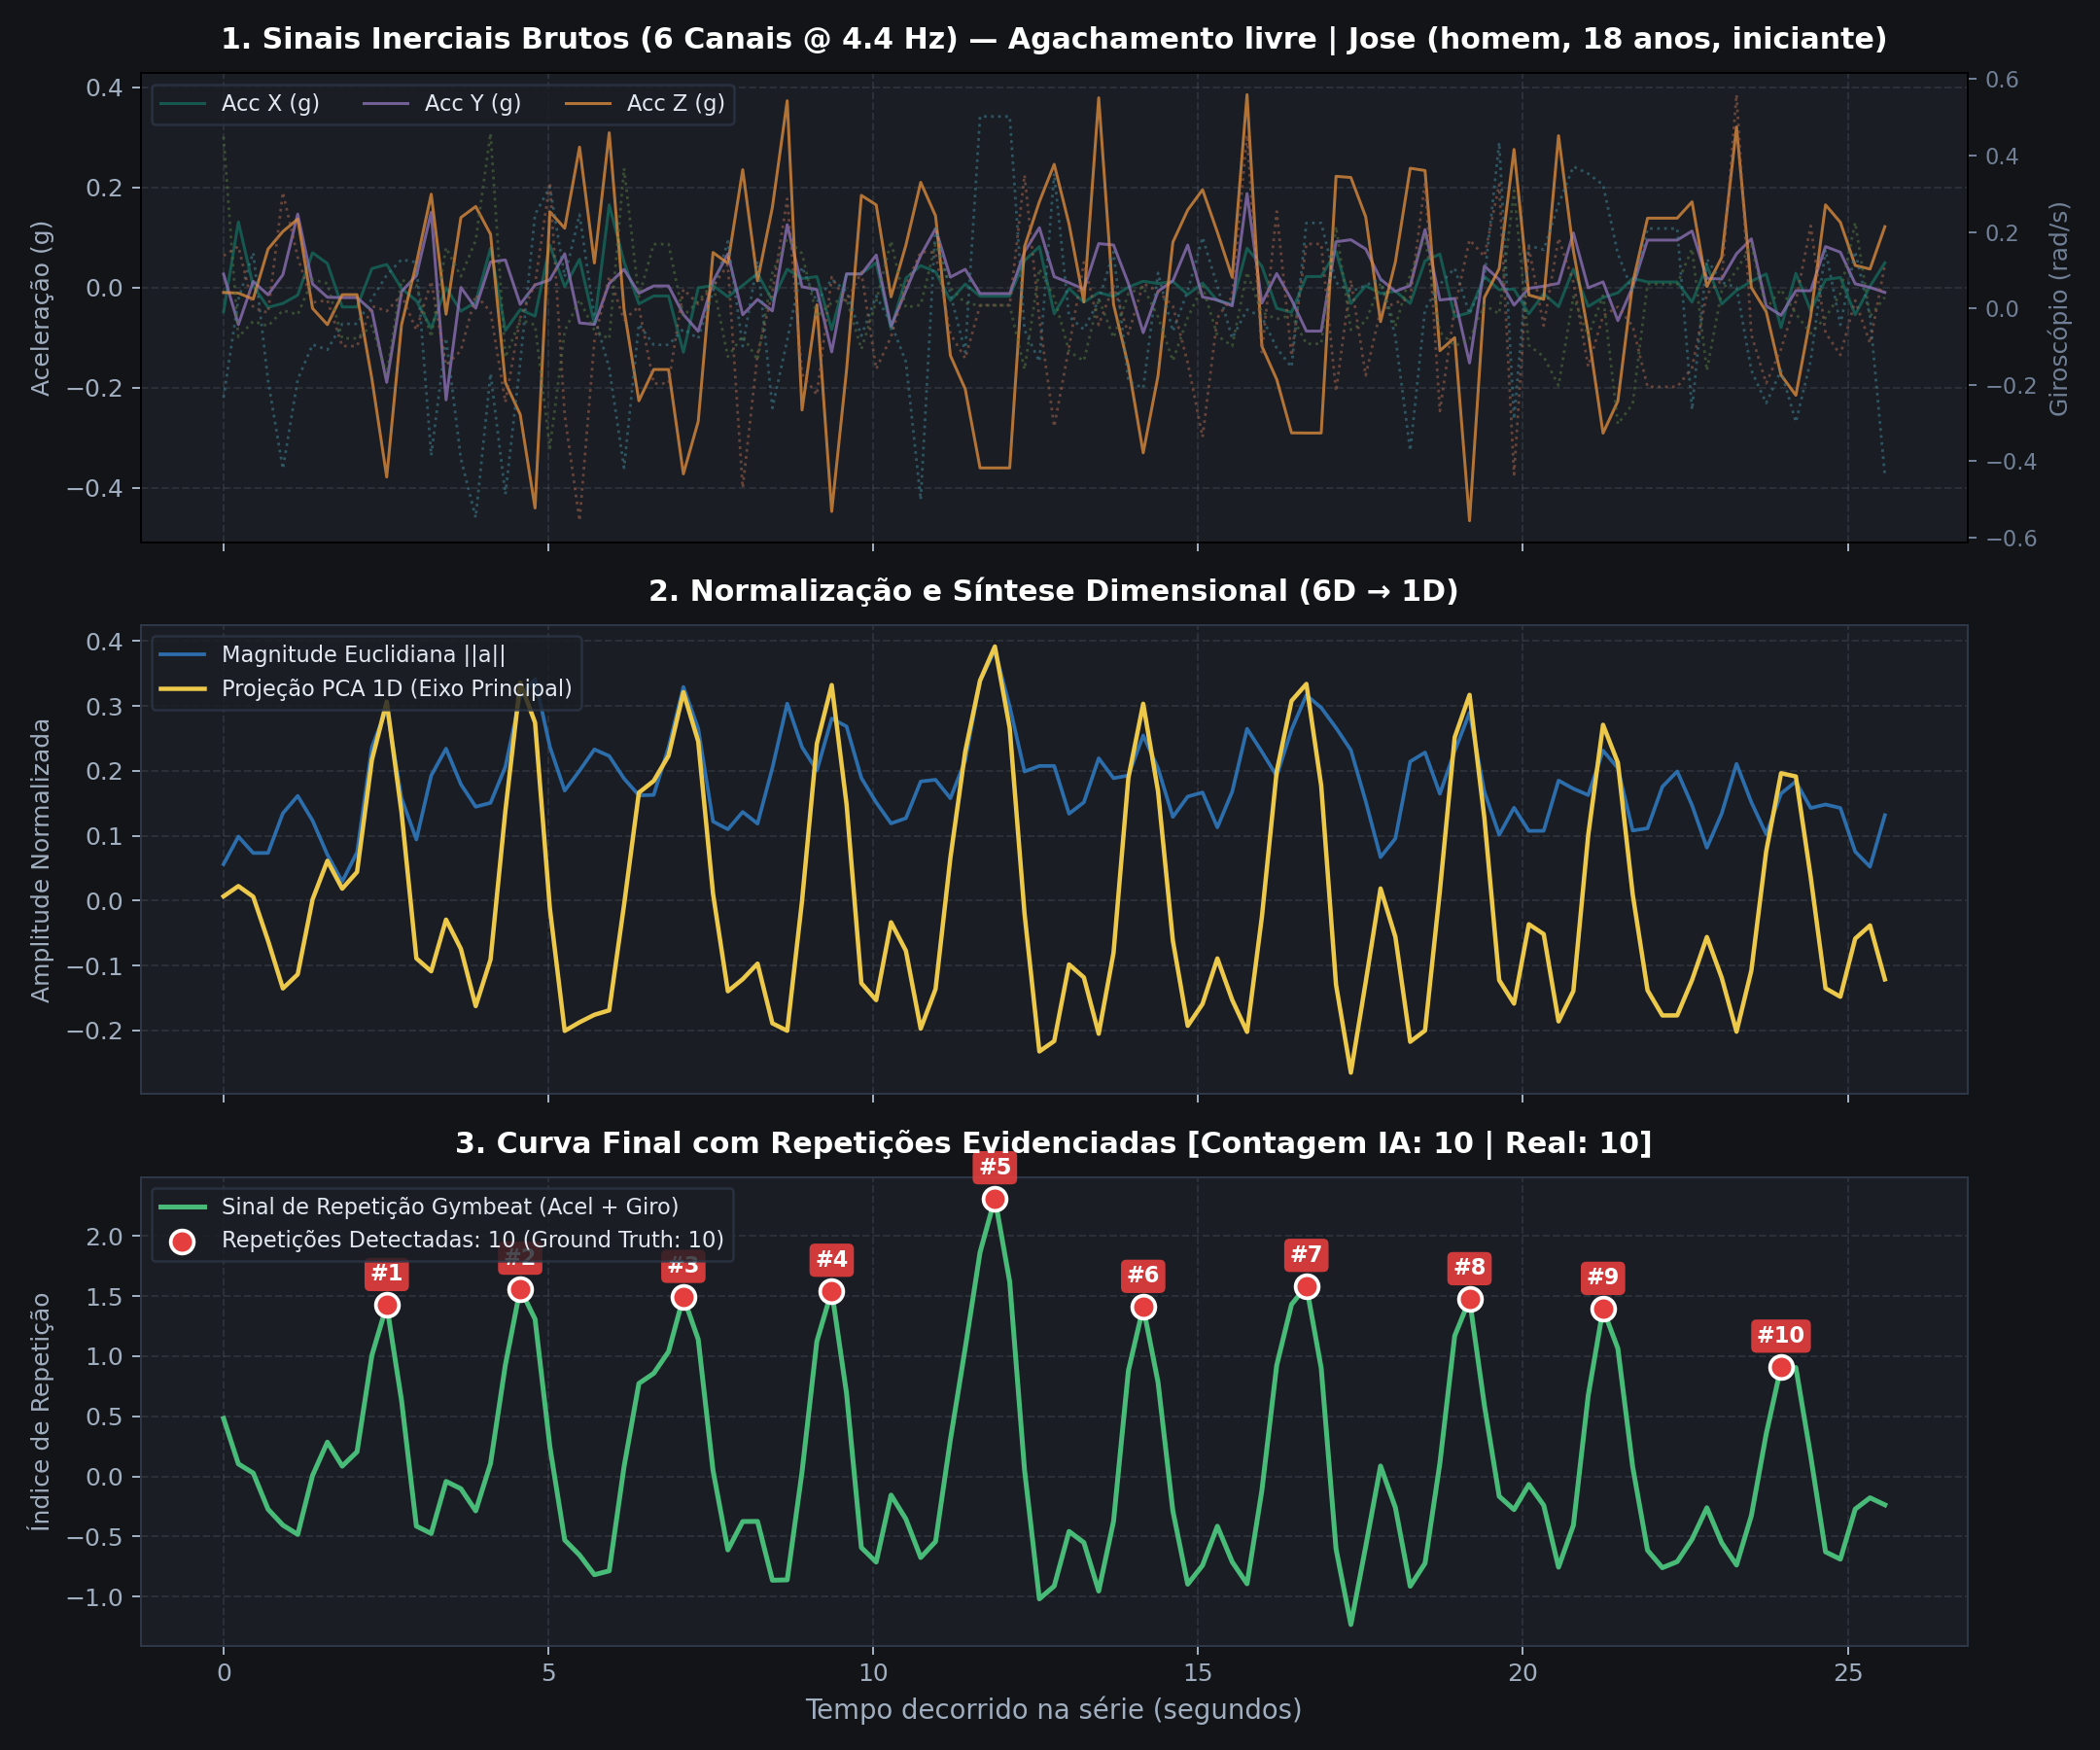
\includegraphics[width=0.92\textwidth]{figuras/grafico_agachamento_sessao1.png}
\caption{Sinal inercial bruto 3D e sinal 1D projetado com picos na Sessão 1}
\label{fig:sessao1}
\end{figure}

\begin{figure}[ht]
\centering
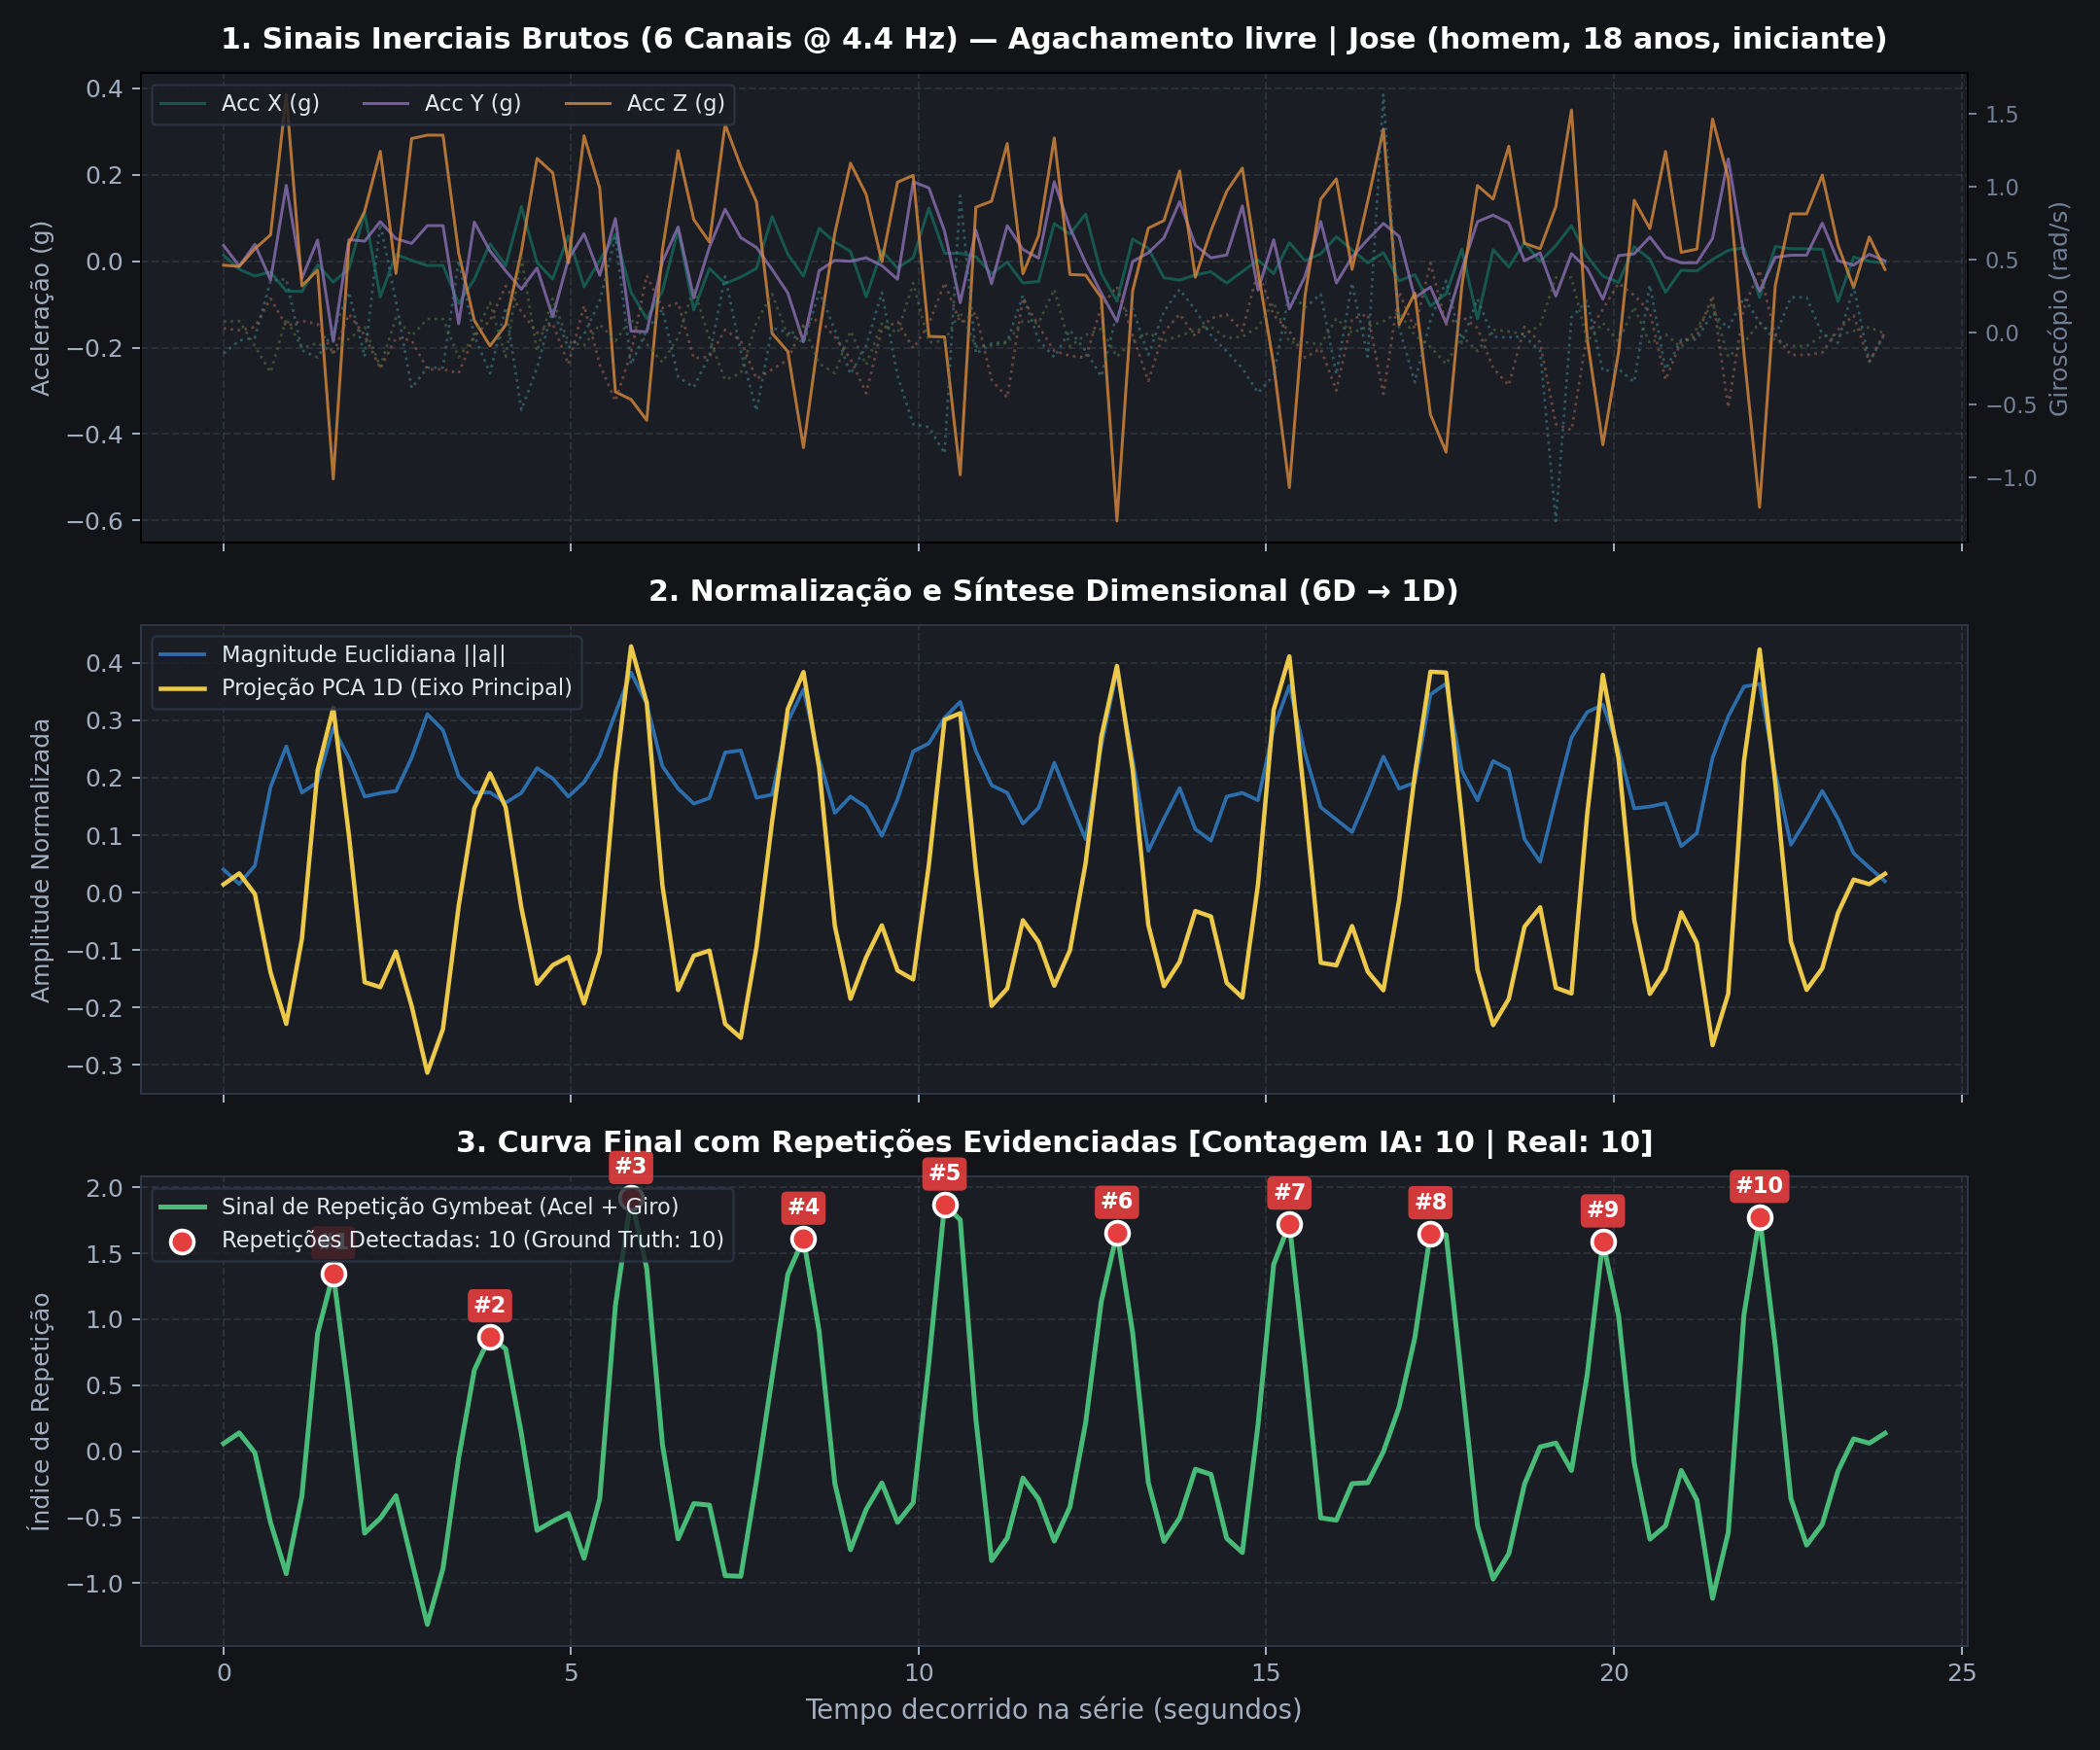
\includegraphics[width=0.92\textwidth]{figuras/grafico_agachamento_sessao2.png}
\caption{Sinal inercial bruto 3D e sinal 1D projetado com picos na Sessão 2}
\label{fig:sessao2}
\end{figure}

O tempo de processamento médio por amostra inercial no motor JavaScript/Hermes foi de apenas $0{,}045\,$ms. O atraso de confirmação temporal total (atraso de grupo do filtro mais 1 amostra de confirmação) foi de aproximadamente $340\,$ms, perfeitamente compatível com o intervalo de transição entre repetições ($\approx 0{,}8\,$s).

\section{Conclusão e Trabalhos Futuros}

O sistema Gymbeat demonstrou que a formulação analítica baseada em Moving PCA, alinhamento por assimetria e filtragem causal IIR biquad viabiliza contagem de repetições com $100\%$ de exatidão e latência de frações de microssegundo em dispositivos móveis convencionais. Como trabalhos futuros, prevê-se a expansão para Treinamento Baseado em Velocidade (VBT) e análise de simetria postural.

\bibliographystyle{sbc}
\bibliography{monografia}

\end{document}
